%==========================
% Chapter 6: Representation Learning: What Transformers Actually Learn
%==========================

\chapter[Representation Learning]{Representation Learning: What Transformers Actually Learn}
\label{ch:representation_learning}

\vspace{1em}

In Chapter 5, we understood transformers as conditional compressors that minimize expected codelength. We saw how attention routes information through dot product similarity, how autoregression breaks sequences into incremental predictions, and how the entire architecture follows naturally from the goal of assigning high probability to likely continuations.

But here is the deeper question: when a model learns to compress text well, what internal structures emerge? What patterns does it discover? If you train a transformer on billions of tokens, optimizing nothing but predictive accuracy, what representations does it build along the way?

This chapter explores what transformers actually learn through the lens of information theory, with an information-geometry view when it clarifies the picture. We will see that useful representations are not accidental byproducts of training: when prediction is hard and capacity is limited, training pressure pushes internal states toward structure that makes prediction easier. Understanding these structures helps explain why transformers transfer so well, where their capabilities come from, and how to use them effectively in practice.

One concrete geometric anchor will recur: at each position, a hidden state $h_t$ is mapped (via a linear head and $\softmax$) to a probability distribution over the vocabulary. These predictive distributions live on a probability simplex, and divergences like KL provide a natural notion of ``distance'' between what two representations predict. In that sense, representation learning can be viewed as learning a good coordinate system for navigating the space of predictive distributions.

\vspace{2em}

\begin{keyinsight}
Representations are shaped by compression pressure. When a model is forced to route rich inputs through limited channels while preserving what matters for prediction, gradient descent pushes it toward encodings that capture stable structure and discard nuisance detail. This is not magic; it is the economics of information under constraints.
\end{keyinsight}

\vspace{2em}

%==========================
\section[From Compression to Structure]{From Compression to Structure:\\Why Representations Emerge}
\label{sec:compression_to_structure}
%==========================

\vspace{1em}

\subsection{The Bottleneck Principle}

A transformer processes a length-$L$ sequence as $L$ vectors in a fixed-width residual stream. At each position, information flows through a vector of dimension $d$ (typically 768, 1024, or larger). The model therefore has $L\cdot d$ degrees of freedom across the whole sequence, but only $d$ degrees of freedom \emph{per position}.

For next-token prediction, the per-position constraint matters most: to predict the next token at position $t$, the model ultimately must distill the relevant context into the single vector $h_t \in \mathbb{R}^d$ that feeds the language-model head. Attention lets $h_t$ \emph{retrieve} information stored at other positions, but what can be made available to the head is still limited by the width of the channels into $h_t$ and by $d$ itself. This creates a bottleneck in the only place that directly affects prediction: the representation at the predicting position.

That bottleneck creates pressure for structure. The model does not need to erase token identity or ``forget'' context; rather, it cannot preserve \emph{all} details with equal fidelity. It must prioritize: compress away nuisance variation while keeping the features that most reduce prediction error. Over training, this pressure tends to yield representations that align with real regularities in the data (syntax, semantics, discourse), because those regularities provide reusable predictive signal.

\vspace{1em}

Formally, this connects to the information bottleneck (IB) objective from Chapter 3. Let $X$ be the context (tokens seen so far), let $Z$ be the representation used for prediction (a hidden state), and let $Y$ be the next token. Because $Z$ is computed from $X$, we have the Markov structure $Y \leftarrow X \rightarrow Z$, and by the data processing inequality $I(Z;Y) \le I(X;Y)$. The IB principle says: keep $Z$ as small as possible while retaining predictive information about $Y$.

In mathematical terms:
\begin{equation}
\min_{p(z|x)} I(X; Z) \quad \text{subject to} \quad I(Z; Y) \geq I_{\min}
\end{equation}

We want a compressed representation $Z$ that still preserves enough information to predict $Y$. Importantly, standard transformer pretraining does not literally optimize this IB constrained problem (mutual information is subtle to define and estimate in high-dimensional deterministic networks). Treat IB as a conceptual scaffold: it explains \emph{why} there is pressure to discard irrelevant detail and keep predictive structure, even when the training objective is simply next-token cross-entropy.

\vspace{1.5em}

\begin{examplebox}
\textbf{Worked Example: Color Compression}

Imagine a task where you see sequences of colored objects and must predict the next color. The input space is high-dimensional: each object has a precise RGB value with millions of possibilities.

\vspace{0.5em}

A naive representation might store exact RGB values: $(143, 201, 87)$, $(139, 205, 91)$, $(148, 198, 84)$. But if the prediction task only depends on broad color categories, this precision is wasted. The model will converge to representations that discretize colors into categories: ``green,'' ``red,'' ``blue.''

\vspace{0.5em}

Why? Because precise RGB values contain information (high $I(X; Z)$) but most of that information is irrelevant for prediction (low $I(Z; Y)$ per bit of $Z$). Compression pressure favors representations that extract the relevant structure (color category) and discard the irrelevant details (exact shade).

\vspace{0.5em}

This is a simplified analogue of what happens in transformers, but with linguistic structure instead of colors. The model learns representations that capture syntactic role, semantic meaning, and contextual relevance while discarding surface details that do not matter for prediction.
\end{examplebox}

\vspace{1.5em}

\begin{figure}[t]
\centering
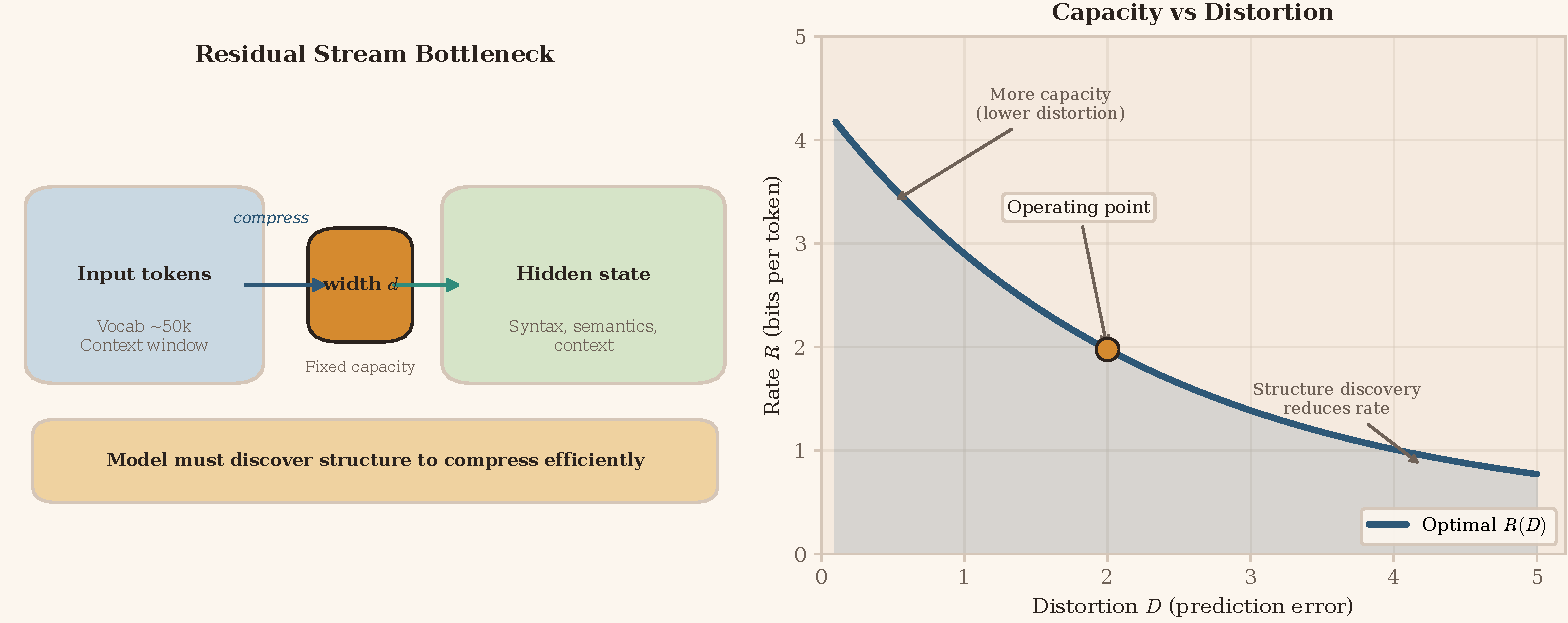
\includegraphics[width=\linewidth]{code/figures/ch06_representation_learning/fig_6_1_bottleneck_principle.pdf}
\caption{A per-position bottleneck in transformers. Attention aggregates context, but the predictive head ultimately sees a single vector $h_t$ of width $d$. Limited capacity forces the model to compress away nuisance detail and preserve the features that most reduce prediction error.}
\label{fig:bottleneck_principle}
\end{figure}

\vspace{1.5em}

\vspace{1.5em}

\subsection{Why Structure Emerges: The Rate-Distortion Perspective}

Rate-distortion theory, introduced in Chapter 1, gives us another lens on why representations have structure. The model faces a tradeoff: it can use more bits (higher rate) to encode context more precisely, or it can use fewer bits (compression) at the cost of some prediction error (distortion).

Strictly speaking, ``rate'' is measured in bits, not in dimensions. Here we use $d$ as a proxy for effective representational capacity: with fixed width (and finite precision / noise / regularization), there is only so much information that can be made reliably available for prediction at each position. Given this budget, the model must choose what to encode. It allocates capacity to features that reduce prediction error the most. Features that matter rarely or contribute little to prediction get encoded more coarsely or dropped.

\vspace{0.5em}

A useful mental model is that each layer communicates through $d$ noisy real-valued channels. Two hidden states that differ only in tiny decimals are effectively indistinguishable to downstream computation once you account for finite precision, stochasticity, and the roughness of optimization. Under this approximation, each dimension carries some finite number of \emph{effective} bits, so increasing $d$ increases the total usable rate by adding more parallel channels. This is why it makes sense (at a high level) to treat width as an information budget even though the underlying math uses bits.

This creates a natural hierarchy. The most important regularities, the patterns that appear frequently and matter most for prediction, get dedicated representational resources. Less important patterns get encoded more coarsely or merged together. Very rare patterns might not be represented explicitly at all, reconstructed on demand from more general features.

\vspace{1em}

Here is the key insight: structure in representations tends to reflect structure in the data, filtered through what matters for prediction. If syntax reliably reduces next-token uncertainty, training pressure will encourage syntactic features. If semantic relationships matter, training pressure will encourage semantic features. The representations are not random; they are shaped by an optimization problem, even if the mapping from objective to learned ``features'' is not unique.

\vspace{1.5em}

\begin{geometrylens}
Think of the space of all possible representations as a high-dimensional manifold. Most points on this manifold correspond to useless representations that predict poorly. But there is a low-dimensional submanifold of good representations that capture the true structure of language. Training via gradient descent on compression loss is a trajectory through this space, pulled toward the good submanifold by the information geometry of the prediction task. The model does not "choose" to learn syntax or semantics; it is drawn there by the loss function and its gradients.
\end{geometrylens}

\vspace{1.5em}

\begin{figure}[t]
\centering
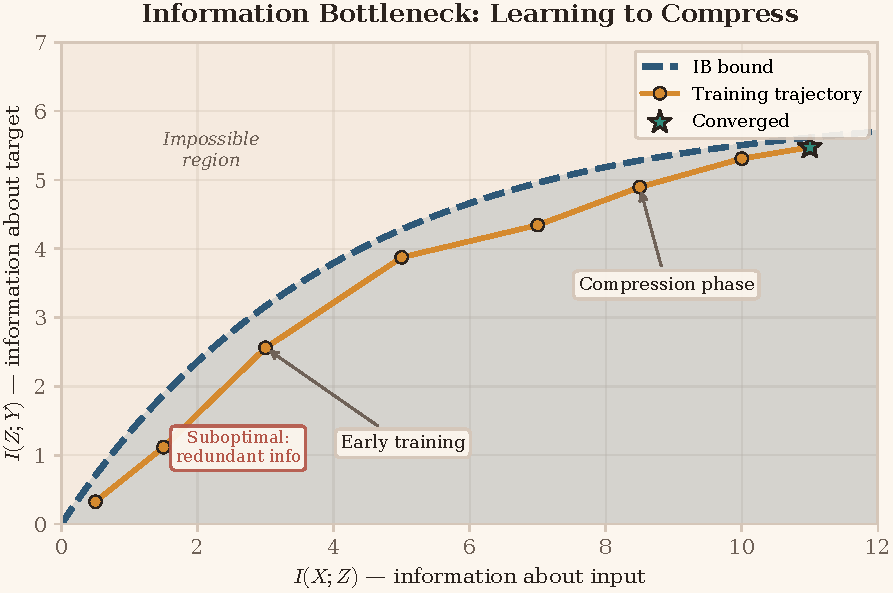
\includegraphics[width=\linewidth]{code/figures/ch06_representation_learning/fig_6_3_information_bottleneck.pdf}
\caption{Rate--distortion tradeoff for prediction: reducing distortion requires allocating more representational rate (capacity). Compression pressure pushes models toward points on the frontier that preserve predictive information while discarding irrelevant detail.}
\label{fig:ib_tradeoff}
\end{figure}

\vspace{1.5em}

\vspace{1.5em}

\subsection{Predictive Information and Sufficiency}

What exactly makes a representation good? From an information-theoretic perspective, a representation $Z$ of input $X$ is useful to the extent that it preserves information that helps predict the target $Y$, while discarding variation that does not.

This is captured by the concept of sufficiency. A representation $Z$ is sufficient for predicting $Y$ if:
\begin{equation}
I(X; Y) = I(Z; Y)
\end{equation}

Equivalently (and often more intuitively), $Z$ is sufficient if conditioning on $Z$ makes the input $X$ irrelevant for predicting $Y$: $Y \perp X \mid Z$, i.e., $p(y\mid z)=p(y\mid x)$ for all $x$ that map to the same $z$. The mutual-information form is a compact summary, but remember that in deterministic, continuous networks mutual information depends on how you model noise or discretization, so treat sufficiency as an \emph{ideal target} and the estimates as practical proxies.

When $Z$ is computed from $X$, we have $Y \leftarrow X \rightarrow Z$ and thus $I(Z;Y) \le I(X;Y)$ by the data processing inequality. Sufficiency is the limiting case where the representation loses no predictive information: knowing $Z$ is as good as knowing $X$ for predicting $Y$.

Minimal sufficiency goes further: $Z$ is minimally sufficient if it is sufficient and no smaller representation could also be sufficient. This is the ideal: the most compressed encoding that loses no predictive power.

In practice, trained transformers exhibit \emph{selective compression}: as depth increases, some information about surface form becomes less directly recoverable, while information useful for next-token prediction remains accessible. How close any given model gets to an IB-style ``minimal sufficient'' representation is an empirical question (and depends on how information is defined/estimated), but the qualitative pressure is clear: limited capacity encourages the model to spend representational budget on what reduces prediction loss.

\vspace{1em}

This helps explain why pretrained representations transfer so well. If pretraining has encouraged representations that emphasize stable, predictive regularities of text, those representations will often be useful across many downstream tasks, even when the tasks differ, because they encode reusable structure rather than task-specific labels.

\vspace{2em}

Take a breath here. We have seen why training a predictive compressor under capacity constraints creates strong pressure for structured representations. The model is incentivized to discover patterns that reliably reduce uncertainty. In the next section, we will see how this structure is often organized across layers, creating a hierarchy of abstraction.

\vspace{2em}

%==========================
\section{Layer-by-Layer Information Flow: The Hierarchy of Abstraction}
\label{sec:layer_hierarchy}
%==========================

\vspace{1em}

\subsection{Early Layers: Surface Statistics}

The first few layers of a transformer operate close to the token embeddings. They see raw vocabulary indices wrapped in positional information. What do they learn?

Early layers tend to capture surface-level statistics. They encode information like token frequency (common words versus rare words), local context (the word before or after), and simple pattern matching (repeated tokens, basic punctuation rules). These representations are relatively concrete and tied to the surface form of the input.

From a compression perspective, this makes sense. Early layers handle the first-order regularities: the easy predictions that require little abstraction. "The" is usually followed by a noun. Punctuation appears in predictable positions. Capitalization signals sentence boundaries. These patterns are statistically strong and can be captured without deep reasoning.

Early layers also begin to build contextualized representations. Unlike static word embeddings, transformer representations depend on context. The representation of "bank" in "river bank" differs from "bank" in "savings bank" even at layer 1 or 2, because attention begins to route information based on surrounding words.

\vspace{1.5em}

\begin{figure}[t]
\centering
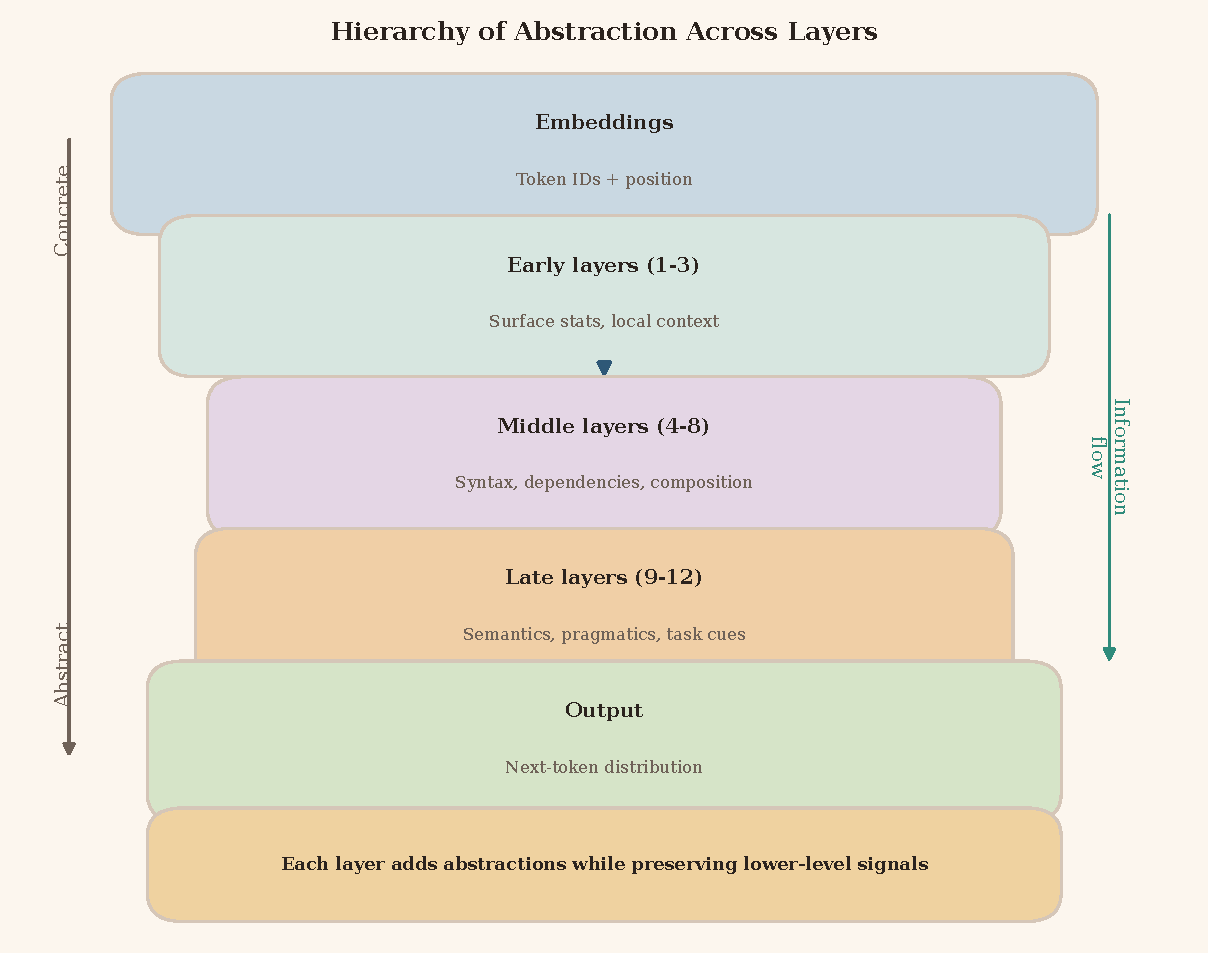
\includegraphics[width=\linewidth]{code/figures/ch06_representation_learning/fig_6_2_layer_hierarchy.pdf}
\caption{Hierarchy of abstraction across layers. Early layers capture surface statistics and local context, middle layers encode syntactic and compositional structure, and late layers form semantic abstractions used for prediction. Each layer adds new abstractions while preserving useful lower-level features.}
\label{fig:layer_hierarchy}
\end{figure}

\vspace{1.5em}

\vspace{1.5em}

\subsection{Middle Layers: Compositional Structure}

As we move deeper into the network, representations often become more abstract. In many architectures, ``middle'' layers (for example, mid-depth in a 12-layer model) tend to make syntactic and compositional structure more directly accessible, though the precise layer boundaries vary by model family, scale, and training data.

For example, middle layers track subject-verb-object relationships. They know that "cat" is the subject of "chased" in "The cat chased the mouse." They encode coreference: "it" refers back to "cat." They capture phrasal meaning: "kick the bucket" is an idiom, not a literal action about buckets.

This compositional structure emerges because it is highly useful for compression. You cannot predict well by treating every multi-word sequence as independent. Language has recursive, hierarchical structure, and models benefit from capturing that structure to generalize. A phrase like "the big red ball" has internal organization: adjectives modify the noun, and that organization affects what comes next.

\vspace{1em}

From an information-theoretic perspective, middle layers can be viewed as performing lossy compression of syntactic and compositional structure. The model does not explicitly represent parse trees (it has no symbolic parser), but its continuous representations can encode much of the information that a parse tree would provide. In many models, some attention patterns correlate with dependency-like relations, while the residual stream carries compositional semantic information.

\vspace{1.5em}

\begin{examplebox}
\textbf{Worked Example: Tracking Syntactic Dependencies}

Consider the sentence: "The chef who prepared the meal received praise."

\vspace{0.5em}

In early layers, each word has a representation that captures its local context. "Prepared" is near "chef" and "meal."

\vspace{0.5em}

In middle layers, attention begins to enforce syntactic structure. The representation of "received" attends strongly to "chef" (the subject) even though they are separated by a relative clause. The model learns that "who" signals a dependency arc back to "chef," and this information propagates through the residual stream.

\vspace{0.5em}

When predicting what comes after "received," the model needs to know the subject is "chef," not "meal." Middle layers encode this by building a representation where "received" is linked to "chef" in the hidden state, capturing the syntactic dependency.

\vspace{0.5em}

This happens without explicit supervision. The model learns syntactic structure purely from the compression objective, because respecting syntax reduces prediction error.
\end{examplebox}

\vspace{1.5em}

\subsection{Late Layers: Semantic Abstractions}

The final layers of a transformer operate at the highest level of abstraction. They encode semantic meaning, pragmatic intent, and task-relevant information. Representations in late layers are far removed from surface form.

Late layers answer questions like: What is this sentence about? What is the speaker's intent? What knowledge is relevant for continuing this text? They aggregate information from across the sequence, building integrated representations that support generation or classification.

For generation tasks, the final layer's output feeds into the language modeling head that predicts the next token. To do well, it must make available the information most relevant for that prediction: topic, style, and the semantic trajectory of the text. It is a high-pressure summary: a single vector per position that must support accurate next-token probabilities.

\vspace{1em}

This layered hierarchy is a common consequence of optimization dynamics. Deep networks often form hierarchies because gradients flow differently at different depths. Early layers receive gradients that reflect immediate prediction errors, such as local, surface-level mistakes. Late layers receive gradients filtered through many nonlinearities, reflecting higher-order, abstract errors. The network structure shapes what each layer can learn.

\vspace{1.5em}

\begin{geometrylens}
Each layer performs a step along a manifold in representation space, moving from concrete token-level encodings toward abstract task-level representations. This trajectory is not arbitrary; it follows the gradients of the compression loss, which pull the representation toward a region of the manifold where prediction is easy. Residual connections make it easier for each layer to add new abstractions while preserving lower-level features that might still matter.
\end{geometrylens}

\vspace{1.5em}

\subsection{The Role of Residual Connections}

Residual connections make this kind of layered organization much easier to learn. Without residuals, deep stacks must repeatedly re-encode everything through nonlinear transformations, which makes optimization harder and can cause useful signals to be washed out. With residuals, each layer can behave like a refinement: start from the current representation and add an update that improves prediction.

This creates an information highway. If a low-level feature is already useful, later layers can keep it (by leaving it mostly unchanged) while adding new abstractions on top. Residuals do not \emph{guarantee} that nothing is forgotten, but they make ``preserve + edit'' the path of least resistance during training.

From a compression perspective, this means different depths can specialize. Early layers can emphasize surface statistics, middle layers can build compositional structure, and late layers can aggregate semantics, while multiple levels of structure can coexist in the residual stream when they remain useful.

\vspace{2em}

Pause and reflect. We have seen that transformers build a hierarchy of abstraction, with early layers handling surface form, middle layers capturing structure, and late layers encoding semantics. This hierarchy emerges naturally from the compression objective and the gradient flow through depth. Next, we zoom in on attention heads to see how they specialize within this hierarchy.

\vspace{2em}

%==========================
\section{Attention Heads as Specialized Feature Detectors}
\label{sec:attention_specialization}
%==========================

\vspace{1em}

\subsection{Multi-Head Attention as Parallel Specialists}

Recall from Chapter 5 that multi-head attention runs multiple attention operations in parallel, each with its own query, key, and value projections. This architectural choice is not arbitrary. It allows different heads to specialize in different aspects of the compression task.

Some heads focus on short-range dependencies: attending to the previous token or nearby words. Others focus on long-range dependencies: connecting distant tokens across the sequence. Some heads are syntactic specialists, tracking grammatical relationships. Others are semantic specialists, linking conceptually related words.

This specialization emerges during training through gradient descent. Different heads receive different gradients depending on what mistakes the model makes. If the model struggles with local coherence, some heads develop strong short-range attention. If it struggles with long-range dependencies, other heads learn to bridge distant positions. The system self-organizes into a collection of specialized modules, each optimized for a different subproblem.

\vspace{1.5em}

\begin{keyinsight}
Multi-head attention is not just a capacity increase; it is a mechanism for functional specialization. By creating multiple parallel information channels, the architecture allows different heads to become experts in different types of dependencies. This modular structure improves both efficiency and interpretability.
\end{keyinsight}

\vspace{1.5em}

\begin{figure}[t]
\centering
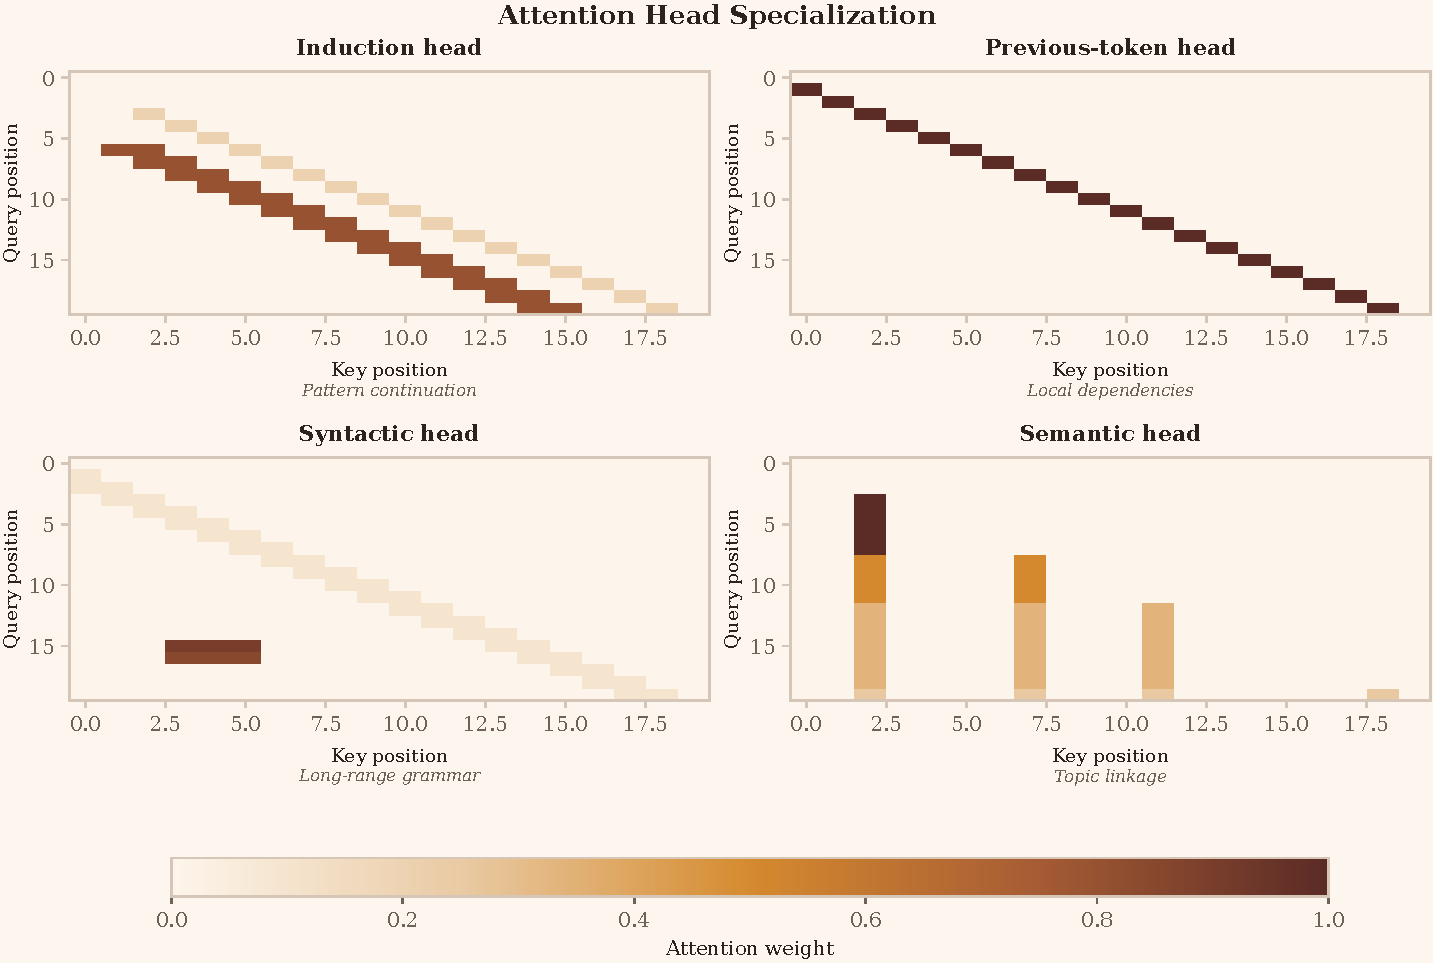
\includegraphics[width=\linewidth]{code/figures/ch06_representation_learning/fig_6_4_attention_specialization.pdf}
\caption{Attention heads specialize. Different heads focus on different dependency types (induction/pattern continuation, previous-token, syntactic, semantic), creating parallel information channels that improve compression and interpretability.}
\label{fig:attention_specialization}
\end{figure}

\vspace{1.5em}

\subsection{Induction Heads: A Canonical In-Context Circuit}

One of the most important and well-studied attention patterns is the induction head. Induction heads detect repeated patterns and continue them. If the model sees "A B ... A," an induction head will attend back to the previous occurrence of A and retrieve what followed (B), allowing it to predict B again.

Induction heads are not the only mechanism behind in-context learning, but they are a canonical circuit for \emph{in-context pattern completion}: using the prompt as a temporary memory and copying a continuation when a key repeats. This can enable some few-shot behaviors within a single forward pass, without parameter updates, especially when the task can be reduced to ``find a repeated key, then copy what came next'' \citep{elhage2021circuits,olsson2022icl}.

From an information-theoretic perspective, induction heads implement a form of compression through pattern matching. Instead of memorizing every possible sequence, the model learns to recognize that sequences contain repeated structures. When it encounters a familiar pattern, it retrieves the cached continuation rather than recomputing from scratch. This is far more efficient than treating every sequence as novel.

\vspace{1.5em}

\begin{examplebox}
\textbf{Worked Example: Detecting Induction}

Consider a toy token sequence where repetition directly determines the next token:
\[
  \texttt{foo\ bar\ baz\ foo}
\]
When the model reaches the second \texttt{foo}, the statistically likely continuation is \texttt{bar} because earlier we saw \texttt{foo} followed by \texttt{bar}.

\vspace{0.5em}

An induction head implements a simple algorithm: attend from the current token (the second \texttt{foo}) back to the previous occurrence of the same token (the first \texttt{foo}), then use the value stream to pull in information correlated with the \emph{next} token after that earlier occurrence (here, \texttt{bar}). In practice this is often realized by a small multi-head circuit (e.g., ``find the match'' plus a position-shift), but the high-level effect is the same: retrieve the continuation when a key repeats. Downstream layers can then translate that retrieved signal into a higher logit for \texttt{bar}.

\vspace{0.5em}

The attention pattern looks like this: at the second \texttt{foo}, the head places high weight on the first \texttt{foo}. This is not hardcoded; it emerges because this ``copy-the-continuation'' strategy reduces loss on sequences with repeated local structure. In real text, the same motif can support behaviors like completing repeated multi-token phrases (e.g., ``New York \ldots New'' $\rightarrow$ ``York'') and other prompt-local copying.

\vspace{0.5em}

In some decoder-only models, induction-like heads often appear in early-to-middle layers, but their prevalence and exact placement vary with architecture and scale. They provide a concrete, mechanistic example of how a model can exploit the prompt as an information source, but many in-context behaviors likely rely on additional circuits beyond pure induction.
\end{examplebox}

\vspace{1.5em}

\begin{figure}[t]
\centering
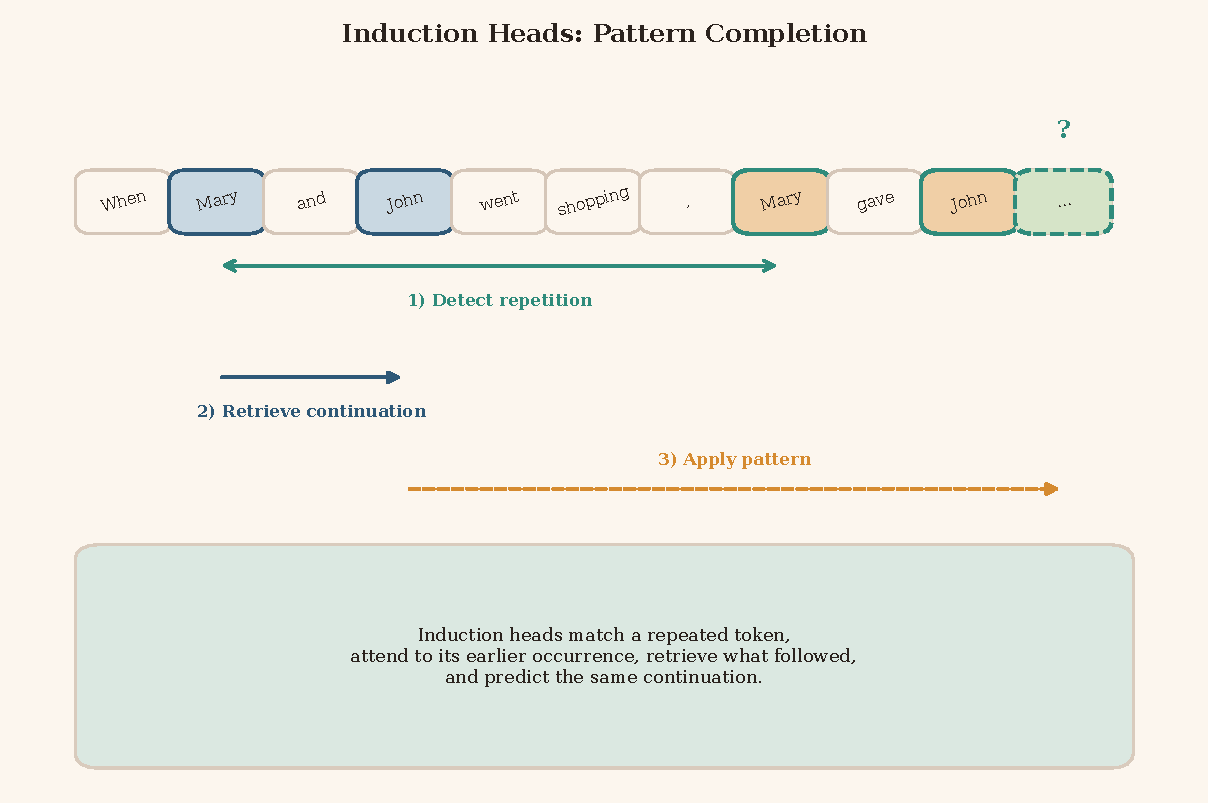
\includegraphics[width=\linewidth]{code/figures/ch06_representation_learning/fig_6_5_induction_heads.pdf}
\caption{Induction heads implement a copy-the-continuation circuit: when a token repeats, the head attends to the previous occurrence and retrieves what followed it, boosting the probability of the same continuation.}
\label{fig:induction_heads}
\end{figure}

\vspace{1.5em}


\vspace{1.5em}

\subsection{Syntactic Heads: Tracking Structure}

Another common specialization is syntactic heads. These heads learn to track grammatical relationships: subject-verb agreement, pronoun-antecedent links, phrase boundaries, and dependency arcs.

For example, a syntactic head might consistently attend from a verb back to its subject, even when they are separated by modifiers or clauses. This allows the model to enforce agreement (singular subjects take singular verbs) and assign semantic roles correctly (the subject is the agent, the object is the patient).

Syntactic heads are often reported in middle-ish layers, consistent with the idea that compositional structure becomes especially usable at intermediate depth. Their prevalence and exact placement vary, but the function is consistent: track long-range dependencies that matter for grammatical coherence.

\vspace{1em}

Why does this matter for compression? Because syntax provides efficient compression schemes. If you know the syntactic structure of a sentence, you can predict word order, agreement markers, and case endings with high accuracy. A model that ignores syntax must memorize many more patterns. A model that discovers syntax can generalize efficiently.

\vspace{1.5em}


\vspace{1.5em}

\subsection{Semantic Heads: Bridging Concepts}

Semantic heads attend based on meaning rather than syntax or position. They link words that are conceptually related even when they are far apart in the sequence and syntactically unconnected.

For example, in a long passage about climate change, a semantic head might attend from "emissions" to "carbon dioxide" mentioned several sentences earlier, or from "temperature" to "warming" across paragraph boundaries. These connections help the model maintain topical coherence and access relevant context for prediction.

Semantic heads are often more prominent in later layers, where the model has already built structured representations and now needs to aggregate meaning over longer ranges. As with all layerwise claims, the details vary by architecture and scale, but the qualitative role is stable: bridge conceptually related content to support coherent prediction.

\vspace{1em}

This specialization reflects an information-theoretic pressure. Different types of dependencies compress different aspects of language. Short-range dependencies compress local coherence. Syntactic dependencies compress grammatical structure. Semantic dependencies compress topical and conceptual continuity. By dedicating different heads to different types of compression, the model can achieve better overall compression than any single attention pattern could.

\vspace{1.5em}

\subsection{Entropy and Specialization}

We can quantify head specialization by measuring the entropy of attention distributions. Recall from Chapter 5 that entropy measures how focused or diffuse attention is.

Highly specialized heads tend to have low entropy. They attend sharply to a few specific positions determined by their specialized function. For example, an induction head has low entropy when it locks onto a previous occurrence of the current token. A syntactic head has low entropy when it identifies the subject of a verb.

General-purpose heads have higher entropy. They spread attention more evenly across many positions, aggregating information broadly rather than retrieving specific patterns. These heads often appear in early or late layers, where the task is more about global context than specific pattern matching.

\vspace{1em}

Measuring entropy across heads reveals the functional structure of the model. Plotting entropy by layer and head shows which parts of the network are acting as specialists (low entropy, focused attention) versus generalists (high entropy, diffuse attention). This gives us insight into what the model is computing and how different components divide labor.

\vspace{2em}

Take a moment. We have seen that attention heads specialize in different types of dependencies, including induction for patterns, syntax for structure, and semantics for meaning. This modular organization emerges from the compression objective and creates an interpretable functional structure. Next, we explore a deeper challenge: what happens when the model needs to represent more features than it has dimensions for?

\vspace{2em}

%==========================
\section{Superposition, Polysemanticity, and Capacity Constraints}
\label{sec:superposition}
%==========================

\vspace{1em}

\subsection{The Dimensionality Problem}

Transformers have a fixed-width residual stream: at each position, the hidden state lives in $\mathbb{R}^d$ (typically $d = 768$, $d = 1024$, or $d = 4096$ for large models). Across a context of length $L$, the model maintains $L$ such vectors, so the model is not forced to compress an entire sequence into a single $d$-dimensional point. The bottleneck is again \emph{per position}: whatever matters for predicting at position $t$ must be made available in the $d$ dimensions (and attention channels) of that position's representation.

But how many features does the model need to track? The answer is enormous. Language involves thousands of concepts, syntactic patterns, semantic relationships, and contextual cues. Even if we conservatively estimate the number of relevant features at ten thousand, we have a problem: we need to store ten thousand features in one thousand dimensions.

How can this possibly work? The answer is superposition. The model stores multiple features in the same dimension by representing them as non-orthogonal vectors that interfere with each other. This allows representing more features than dimensions, at the cost of some crosstalk between features.

\vspace{1.5em}

\begin{keyinsight}
Superposition is a principled response to capacity constraints. When there are more potential features than available dimensions, a network can store features as overlapping (non-orthogonal) directions in high-dimensional space. The geometry of the space determines how much interference occurs. This is not necessarily a bug; it can be an efficient tradeoff when sparsity and downstream readout tolerate some crosstalk.
\end{keyinsight}

\vspace{1.5em}

\begin{figure}[t]
\centering
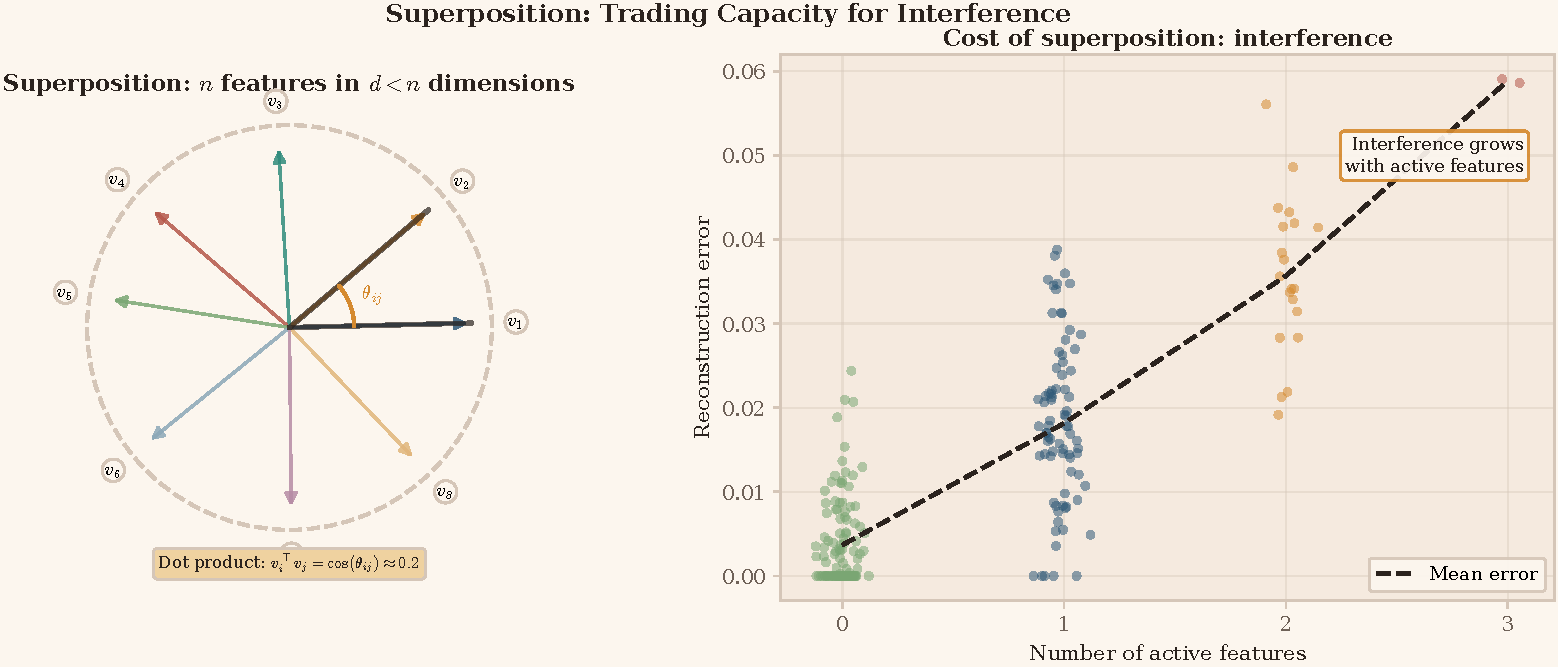
\includegraphics[width=\linewidth]{code/figures/ch06_representation_learning/fig_6_6_superposition.pdf}
\caption{Superposition: many features share the same representational space. Sparse activation allows overlapping feature directions to coexist with manageable interference.}
\label{fig:superposition}
\end{figure}

\vspace{1.5em}

\subsection{How Superposition Works: The Geometry}

Suppose we want to represent $n$ features using $d$ dimensions, where $n > d$. If we require features to be orthogonal, this is impossible; we can have at most $d$ orthogonal vectors in $d$-dimensional space.

But if we relax orthogonality, we can pack more vectors. The key insight is that in high dimensions, there is room for many \emph{almost} orthogonal directions. For example, in $d = 1000$ dimensions, it is often possible to place on the order of thousands of unit vectors with modest overlap (e.g., $|v_i^\top v_j| \lesssim 0.1$). The exact counting depends on what overlap you demand and which regime you care about; we revisit this more carefully in the Notes and Caveats section.

These vectors are not orthogonal, so activating multiple features simultaneously creates interference. If features $i$ and $j$ are both active, their vectors $v_i$ and $v_j$ add, and the result is a point in space that is close to both. When we later probe for feature $i$, we might also detect some signal from feature $j$ due to their non-zero dot product. This is the cost of superposition.

\vspace{1em}

However, if features are sparse, with most features inactive most of the time, this interference is manageable. When only a few features are active simultaneously, their vectors do not collide much. The model can encode many features in superposition and still extract them reliably most of the time.

\vspace{1.5em}


\vspace{1.5em}

\begin{geometrylens}
Think of the representation space as a high-dimensional sphere. Each feature corresponds to a direction (a point on the sphere). Orthogonal features are $90^\circ$ apart. Features in superposition are at angles \emph{less} than $90^\circ$, often still fairly close to orthogonal (small dot products), but not exactly. When multiple features activate, you sum their directions, producing a vector that has components along several feature directions. Linear readouts can recover those components imperfectly, and the nonzero overlaps create crosstalk. This is why superposition can work: high-dimensional geometry admits many directions with small overlaps, and sparsity keeps the number of simultaneously active directions manageable.
\end{geometrylens}

\vspace{1.5em}

\subsection{Polysemanticity: One Neuron, Many Meanings}

Superposition leads to a confusing phenomenon called polysemanticity. A single neuron (or direction in activation space) responds to multiple unrelated features. It is not a clean detector of one concept; it fires for several different concepts that happen to be stored in overlapping directions.

For example, you might find a neuron that activates for both "numbers" and "programming keywords." These concepts are unrelated semantically, but they happen to share representational resources because the model stored them in interfering directions. The neuron is not "about" either concept individually; it is a shared resource used by both.

This makes interpretation difficult. You cannot simply look at individual neurons and assign them clean meanings. Instead, meanings are distributed across combinations of neurons. A feature might be represented by a pattern of activation across many neurons, and those same neurons might also participate in representing other features.

\vspace{1em}

From an information-theoretic perspective, polysemanticity is a signature of lossy compression. The model has accepted some distortion (crosstalk between features) in exchange for higher rate (storing more features). This aligns with a rate--distortion intuition: under capacity constraints, the optimal tradeoff can involve controlled interference.

\vspace{1.5em}

\begin{figure}[t]
\centering
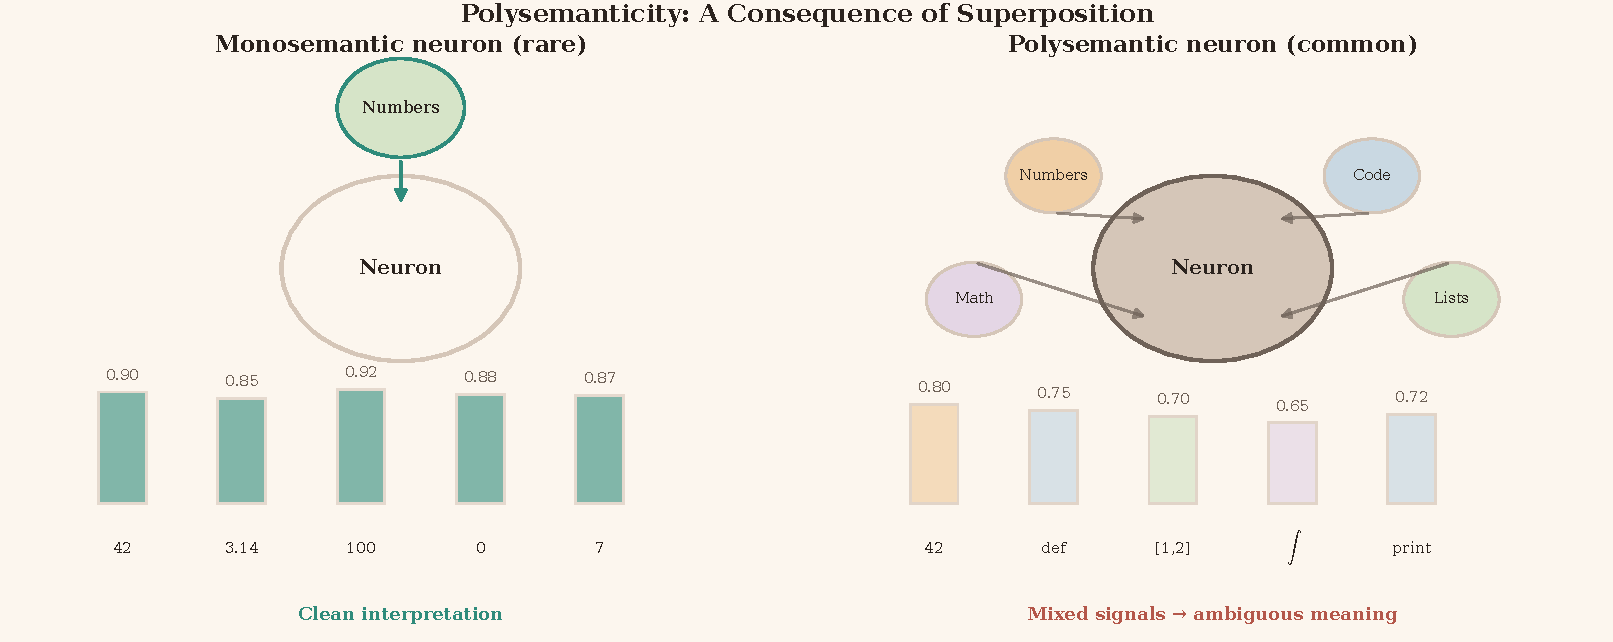
\includegraphics[width=\linewidth]{code/figures/ch06_representation_learning/fig_6_7_polysemanticity.pdf}
\caption{Polysemanticity: a single neuron or direction can respond to multiple unrelated concepts because features are stored in overlapping directions.}
\label{fig:polysemanticity}
\end{figure}

\vspace{1.5em}


\vspace{1.5em}

\begin{examplebox}
\textbf{Worked Example: Identifying Superposition}

Suppose we train a small transformer on a toy task where we know exactly which features matter: capitalization, whether a word is a noun, and whether it is part of a proper name. There are three binary features but only two dimensions available.

\vspace{0.5em}

The model might learn three feature directions:
\begin{align*}
v_{\text{capital}} &= (1, 0) \\
v_{\text{proper}} &= (0, 1) \\
v_{\text{noun}} &= \tfrac{1}{\sqrt{2}}(1, 1)
\end{align*}
These vectors are unit length but not orthogonal: $v_{\text{noun}}$ overlaps with both $v_{\text{capital}}$ and $v_{\text{proper}}$.

\vspace{0.5em}

Suppose the representation is the sum of active feature directions,
\[
r \;=\; x_{\text{capital}}v_{\text{capital}} \;+\; x_{\text{proper}}v_{\text{proper}} \;+\; x_{\text{noun}}v_{\text{noun}},
\qquad x_\cdot\in\{0,1\},
\]
and a simple linear readout for ``noun'' uses the dot product score $s_{\text{noun}} = r^\top v_{\text{noun}}$ (followed by a threshold).

\vspace{0.5em}

If only \emph{noun} is active, then $r=v_{\text{noun}}$ and $s_{\text{noun}} = 1$.
But if \emph{capital} and \emph{proper} are active (and \emph{noun} is not), then $r=(1,1)$ and
\[
s_{\text{noun}} \;=\; (1,1)\cdot \tfrac{1}{\sqrt{2}}(1,1) \;=\; \sqrt{2}\approx 1.41.
\]
A naive threshold would now falsely report ``noun'' as present. This is the core interference problem: overlapping directions create \emph{crosstalk} in simple readouts.

\vspace{0.5em}

In real networks, readouts are learned and can partially compensate for common overlaps, and, crucially, features are often sparse (few co-activate at once). Under sparsity, the occasional crosstalk is an acceptable price for representing more potential features than dimensions.
\end{examplebox}

\vspace{1.5em}

\subsection{Why Models Accept Superposition}

Given the downsides of interference, why do models use superposition? Why not simply use more dimensions and avoid the problem?

The answer is that superposition can be an efficient tradeoff given the constraints. Increasing dimensionality is expensive because it multiplies the number of parameters and the computational cost. For a fixed compute budget, there is a tradeoff between width (more dimensions, less superposition) and depth (more layers, more abstraction).

Empirically, models tend to favor depth over width. Deeper models generalize better because they build hierarchical representations. But depth with narrow layers creates severe capacity constraints, forcing superposition. The model accepts interference as the price of depth.

Moreover, superposition is not always bad. It can improve generalization by forcing the model to share resources between related features. If two features frequently co-occur, storing them in overlapping directions might actually help, because activating one partially activates the other, which can be useful for prediction. Superposition becomes a form of inductive bias toward feature sharing.

\vspace{1.5em}

\begin{pausebox}
\textbf{Pause and Reflect.} Superposition is one of the most surprising findings from mechanistic interpretability. It suggests that models often pack many potential features into a limited residual stream by allowing controlled overlap. You should not read this as a theorem about global optimality, but it is a vivid example of a rate--distortion tradeoff in action: more effective capacity, at the cost of some interference.
\end{pausebox}

\vspace{2em}

%==========================
\section{Measuring Representations: Probes, Projections, and Information Content}
\label{sec:measuring_representations}
%==========================

\vspace{1em}

\subsection{The Problem of Access: Just Because It Is There Does Not Mean You Can Use It}

We have established that transformers learn rich representations. But how do we measure what is encoded? If a model has learned syntactic structure, how do we know? If it represents semantic concepts, how do we prove it?

This is the problem of access. Information might be present in the representations without being easily extractable. A probe might fail to find a feature not because it is absent, but because it is encoded in a way that the probe cannot access. Conversely, a probe might succeed not because the model "understands" the feature, but because the feature is linearly separable by coincidence.

We need principled ways to measure representations that account for this access problem. Information theory provides the framework: we want to measure the mutual information between representations and features of interest, while acknowledging that this information might not be linearly accessible.

\vspace{1.5em}

\subsection{Linear Probing: The Simplest Test}

The most common approach is linear probing. We freeze the model, extract representations from some layer, and train a linear classifier to predict some property from those representations. If the classifier succeeds, we conclude that the property is linearly encoded.

For example, to test if a model encodes part-of-speech tags, we extract hidden states for each token and train a linear classifier to predict whether each token is a noun, verb, adjective, and so on. If the classifier achieves high accuracy, the representations contain linearly accessible part-of-speech information.

Linear probes are useful because they test whether information is accessible to downstream linear layers. If a feature is linearly separable in layer $L$, then subsequent layers can easily use it, since they only need to apply a learned linear projection. This tells us what information is available for the model's own computation.

\vspace{0.5em}

One caution: a probe is an \emph{external} decoder, not the model's own mechanism. High probe accuracy is evidence that a feature is \emph{readable} with low complexity, but it does not, by itself, prove the model is actually using that feature at inference time. We return to this distinction (use vs.\ presence) in the Notes and Caveats section.

\vspace{1em}

\begin{figure}[t]
\centering
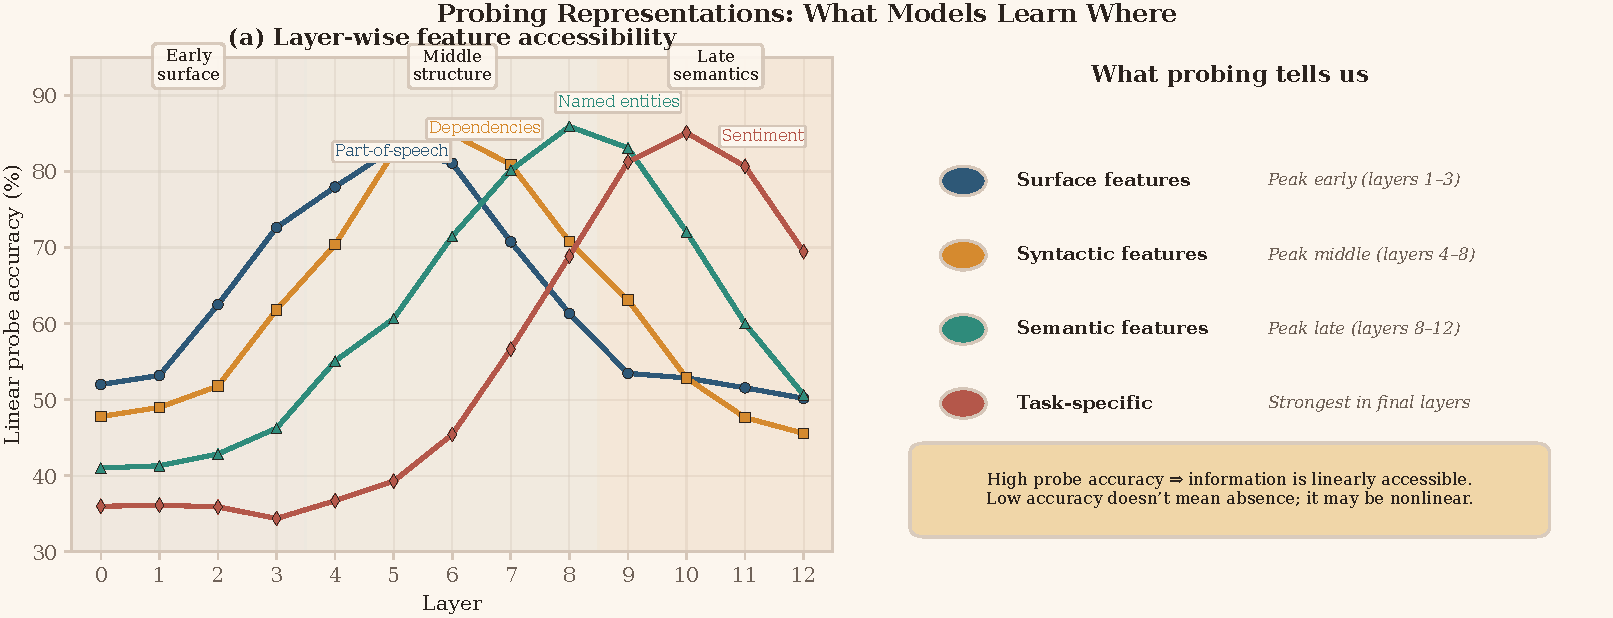
\includegraphics[width=\linewidth]{code/figures/ch06_representation_learning/fig_6_8_probing_accuracy.pdf}
\caption{Probing accuracy across layers often peaks for syntax in middle layers, while semantic probes improve later, reflecting a hierarchy of abstraction.}
\label{fig:probing_accuracy}
\end{figure}

\vspace{1.5em}

However, linear probes have limitations. They only detect linearly separable features. If a feature is encoded nonlinearly (for example, as the product of two hidden dimensions), a linear probe will fail even though the information is present. This creates false negatives: the probe fails, but the model might still be using the feature through nonlinear transformations.

\vspace{1.5em}

\begin{examplebox}
\textbf{Worked Example: Probing for Syntax}

Suppose we want to test if a model encodes syntactic dependencies. We extract hidden states from each layer and train linear probes to predict dependency arcs: for each token, predict which other token is its syntactic head.

\vspace{0.5em}

We find:
\begin{itemize}
\item Layer 1: Probe accuracy 60\% (better than random 10\%, but not great)
\item Layer 4: Probe accuracy 85\% (substantial improvement)
\item Layer 8: Probe accuracy 87\% (marginal further improvement)
\item Layer 12: Probe accuracy 83\% (slight decrease)
\end{itemize}

\vspace{0.5em}

In this toy run, syntactic structure is most linearly accessible in middle layers (here, around layers 4--8), consistent with our earlier qualitative picture. Early layers have not yet built structured representations. Late layers may have transformed syntax into higher-level abstractions that are less linearly separable.

\vspace{0.5em}

Importantly, the probe accuracy being less than 100\% does not mean the model "does not understand" syntax. It means either (a) syntax is encoded nonlinearly, or (b) the model has compressed syntax lossy, retaining only what it needs for prediction. Both are consistent with the model performing well on language modeling.
\end{examplebox}

\vspace{1.5em}


\vspace{1.5em}

\subsection{Nonlinear Probes and Causal Interventions}

To go beyond linear probing, we can use nonlinear probes, which are small neural networks trained to extract features from representations. These can capture more complex encodings, but they come with a new problem: overfitting. A sufficiently large nonlinear probe can memorize the training data without actually extracting structure from the representations.

To control for this, we must carefully validate probes on held-out data and compare their performance to control baselines. If a nonlinear probe performs only slightly better than a linear probe, the nonlinearity might not be capturing genuine structure; it might be overfitting noise.

\vspace{1em}

A more targeted technique is causal intervention. Instead of just measuring what is in the representations, we edit them and measure the effect on model behavior. For example, we might identify a direction in activation space that corresponds to "sentiment" and then ablate (zero out) that direction, observing whether the model's predictions change in the expected way.

If ablating a direction causes the model to lose the ability to distinguish positive from negative text, we have causal evidence that the direction encodes sentiment. This is stronger than correlational evidence from probes, which only tell us that sentiment is predictable from the representations, not that the model actually uses it.

\vspace{1.5em}

\subsection{Mutual Information and Sufficiency Testing}

From an information-theoretic perspective, what we really want to measure is mutual information: $I(Z; Y)$ where $Z$ is the representation and $Y$ is the feature of interest. This quantifies how much information about $Y$ is contained in $Z$, regardless of whether it is linearly accessible.

However, mutual information is notoriously difficult to estimate in high dimensions. Standard estimators can require exponentially many samples in worst cases and are sensitive to noise. Recent work has developed better estimators based on variational bounds and contrastive learning, but estimation remains challenging.

A related concept is sufficiency testing. We ask: does the representation $Z$ contain all the information that the input $X$ provides about $Y$? Formally, is $I(Z; Y) = I(X; Y)$? If so, $Z$ is sufficient, meaning nothing has been lost. If not, we can quantify the information loss: $I(X; Y) - I(Z; Y)$.

\vspace{1em}

Sufficiency testing helps us understand where in the network information is preserved versus compressed away. Early layers typically have high mutual information with input features (low compression). Middle layers compress some features while preserving others (selective compression). Late layers often compress away many features while preserving what remains most predictive (approaching ``minimal sufficiency'' in an idealized sense).

\vspace{1.5em}

\begin{geometrylens}
Measuring representations is fundamentally about mapping the geometry of the representation space. Linear probes test whether a feature is recoverable by a low-capacity linear readout: is there a simple hyperplane (or direction) that separates the labels? Nonlinear probes broaden the readout class, but must be controlled to avoid learning the task from scratch. Causal interventions test whether changing a direction changes behavior. Mutual information aims to summarize total dependence, but is hard to estimate reliably at scale. Each tool reveals a different aspect of how the model has organized its representation space under compression constraints.
\end{geometrylens}

\vspace{2em}

Take a breath. We have seen how to measure what models learn through probing, intervention, and information-theoretic analysis. These tools reveal the structure of learned representations and help us understand what the model has discovered through compression. Finally, we turn to practical implications: how does understanding representations guide us in using models effectively?

\vspace{2em}

%==========================
\section{Implications for Transfer, Fine-tuning, and Adaptation}
\label{sec:practical_implications}
%==========================

\vspace{1em}

\subsection{Why Pretraining Transfers: The Universality of Compression}

Pretrained language models transfer remarkably well to downstream tasks. A model trained only to predict next tokens can be fine-tuned with small amounts of labeled data to perform classification, question answering, summarization, and countless other tasks. Why does this work?

The information-theoretic answer is that compression objectives encourage models to learn broadly reusable features. To compress text well, a model benefits from capturing stable regularities of language, including syntax, semantics, pragmatics, and some world regularities. These are not specific to any particular downstream label; they are general-purpose scaffolding for prediction.

When you fine-tune a pretrained model on a downstream task, you are not teaching it language from scratch. You are teaching it a small task-specific mapping from its already-learned representations to task labels. The hard work of learning to represent language has already been done during pretraining. The task-specific fine-tuning only needs to learn which aspects of the learned representations are relevant for the new task.

\vspace{1em}

This helps explain why fine-tuning often requires far less labeled data than training from scratch. If you train a model from random initialization, you must learn both representations and a task mapping. If you fine-tune a pretrained model, much of the representational work is already done, and you mostly learn how to read out and slightly adjust existing features. In many practical settings, the difference can be orders of magnitude rather than a small constant factor.

\vspace{1.5em}

\begin{keyinsight}
Transfer learning works because compression encourages reuse. The representations learned through unsupervised compression capture broad statistical structure of language, and this structure is useful for many tasks. Fine-tuning is efficient because it often only needs to learn a small task-specific head on top of these reusable representations.
\end{keyinsight}

\vspace{1.5em}

\begin{figure}[t]
\centering
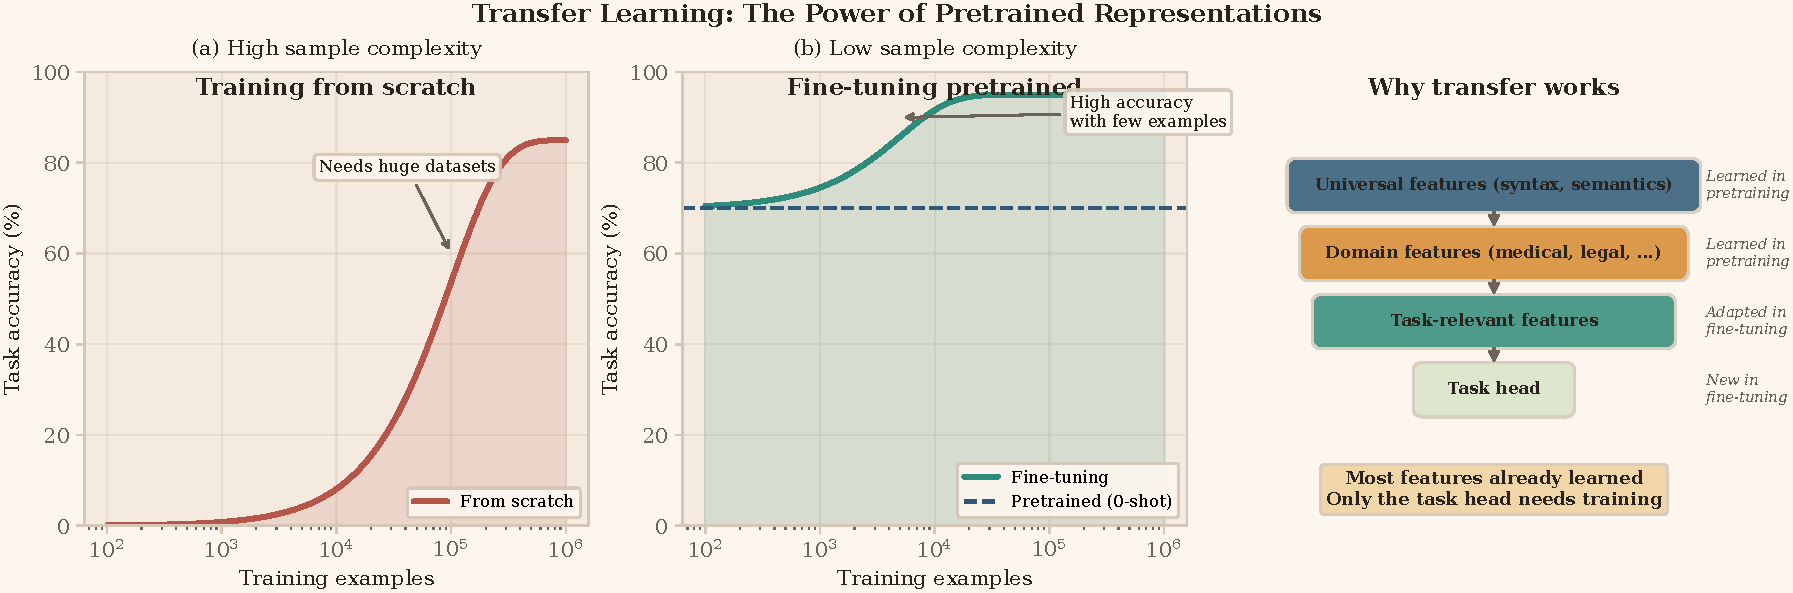
\includegraphics[width=\linewidth]{code/figures/ch06_representation_learning/fig_6_9_transfer_learning.pdf}
\caption{Transfer learning: pretraining builds reusable representations that can be adapted to many downstream tasks with small task-specific updates.}
\label{fig:transfer_learning}
\end{figure}

\vspace{1.5em}


\vspace{1.5em}

\subsection{Where to Fine-Tune: Layer-Wise Decisions}

Understanding the layer-wise hierarchy of representations tells us where to fine-tune for different tasks. Different tasks benefit from intervening at different depths.

Tasks that depend on surface features often benefit from adapting earlier layers. For example, if you are building a text normalizer that needs to fix capitalization and punctuation, you may want to modify early layers where surface statistics are more directly represented. Fine-tuning only late layers might leave those representations mostly unchanged.

Tasks that depend on compositional structure often benefit from adapting intermediate layers. For syntax-heavy tasks like parsing or grammatical error correction, intermediate layers frequently make structure most accessible. Fine-tuning these layers can adjust how the model composes information while leaving early and late layers relatively stable.

Tasks that depend on semantic meaning often benefit from adapting later layers. For classification, summarization, or question answering, task-relevant information is frequently concentrated in late-layer representations. Fine-tuning these layers reshapes how the model aggregates information into task-relevant abstractions.

\vspace{1em}

In practice, the most common approach is to fine-tune all layers but with different learning rates (discriminative fine-tuning). Early layers get small learning rates because they encode universal features that should not change much. Late layers get larger learning rates because they need to adapt more substantially to the new task. This balances preserving pretrained knowledge with task-specific adaptation.

\vspace{1.5em}

\begin{figure}[t]
\centering
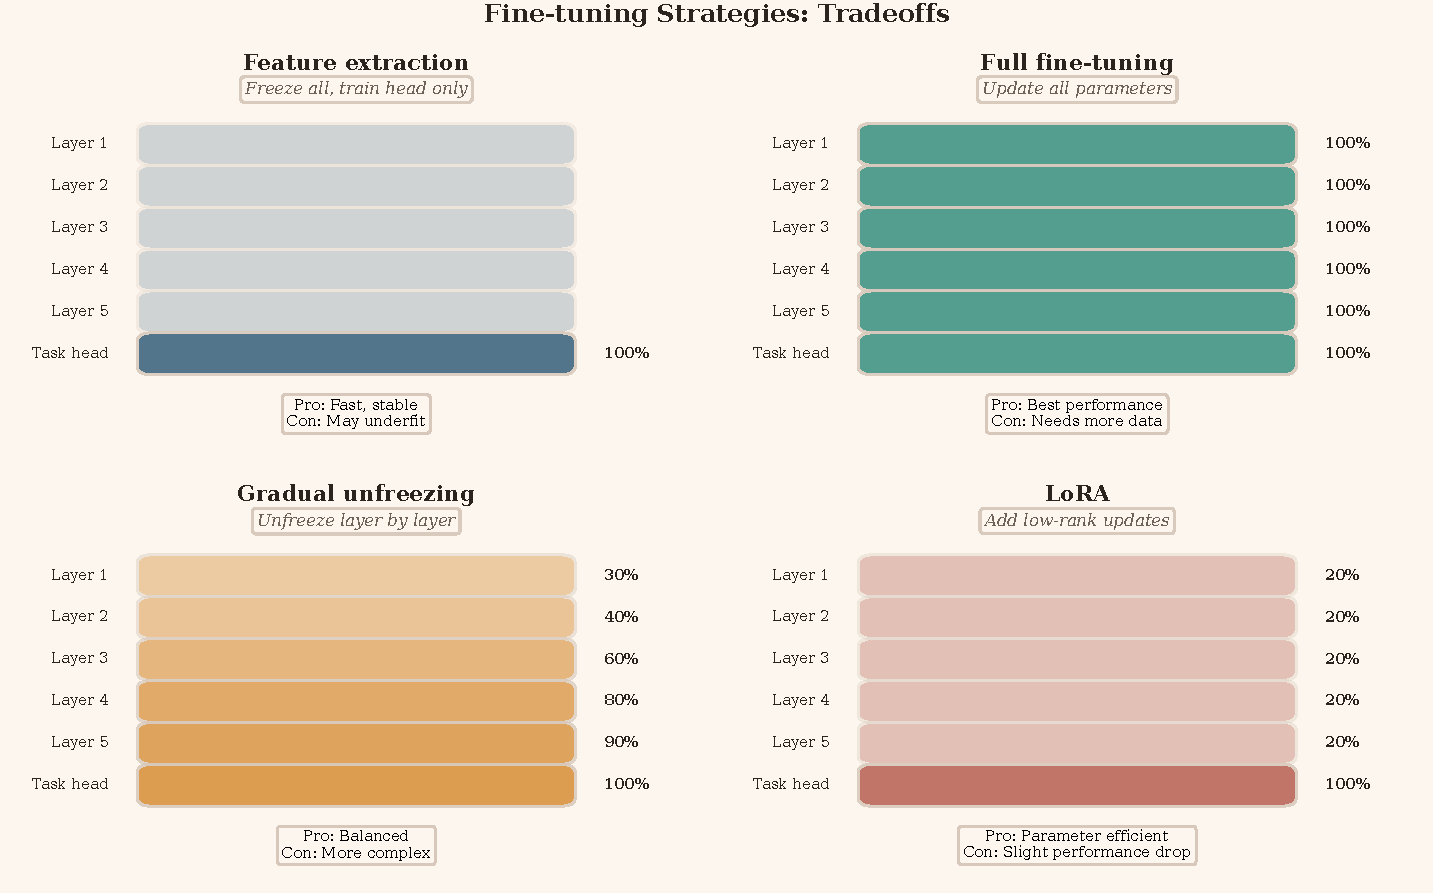
\includegraphics[width=\linewidth]{code/figures/ch06_representation_learning/fig_6_10_finetuning_strategies.pdf}
\caption{Fine-tuning strategies trade off adaptation and stability. Full fine-tuning updates all layers; adapters and LoRA update small parameter subsets to reduce cost.}
\label{fig:finetuning_strategies}
\end{figure}

\vspace{1.5em}

\begin{examplebox}
\textbf{Worked Example: Fine-Tuning for Sentiment Analysis}

Suppose we fine-tune a pretrained model for sentiment classification. We have two choices: fine-tune only the final layer (adding a classification head) or fine-tune all layers.

\vspace{0.5em}

Fine-tuning only the final layer treats the model as a fixed feature extractor. We train a linear classifier on the final-layer representations. This is fast and data-efficient but might underperform if the pretrained representations are not perfectly aligned with sentiment (for example, if the pretraining data was factual text but the fine-tuning data is reviews with emotional language).

\vspace{0.5em}

Fine-tuning all layers allows the model to adjust its representations to emphasize sentiment-relevant features. Early layers might learn to attend more to emotionally loaded words. Middle layers might adjust how they compose phrases to capture sentiment composition ("not bad" is positive despite "bad" being negative). Late layers reshape their semantic representations to separate positive from negative examples.

\vspace{0.5em}

Empirically, full fine-tuning usually performs better, especially with moderate amounts of data (thousands of examples). With very little data (dozens of examples), fine-tuning only the head is safer to avoid overfitting. This is another tradeoff guided by information theory: more parameters to adapt means higher capacity but also higher risk of fitting noise.
\end{examplebox}

\vspace{1.5em}


\vspace{1.5em}

\subsection{Parameter-Efficient Fine-Tuning: LoRA and Beyond}

Full fine-tuning updates all model parameters, which is expensive in memory and compute for large models. Parameter-efficient fine-tuning (PEFT) methods aim to achieve similar performance while updating far fewer parameters.

One of the most successful approaches is LoRA (Low-Rank Adaptation). Instead of updating the full weight matrices, LoRA adds low-rank perturbations. For a weight matrix $W$, instead of learning a full update $\Delta W$, we learn $\Delta W = AB$ where $A$ and $B$ are low-rank matrices (typically rank 4 to 16).

Why does this work? From an information-theoretic perspective, most of the information needed for adaptation lies in a low-dimensional subspace. The pretrained weights already capture most of the structure. The task-specific adaptation only needs to make small adjustments, which can be represented in a low-dimensional space. LoRA explicitly parameterizes this intuition.

\vspace{1em}

Other PEFT methods include adapter layers (small bottleneck modules inserted between transformer layers), prefix tuning (learning soft prompts that modulate behavior), and selective fine-tuning (freezing most parameters and only updating specific components like attention or feedforward layers). Each method makes different tradeoffs between parameter efficiency, task performance, and implementation complexity.

\vspace{1.5em}

\subsection{Prompting Versus Fine-Tuning: An Information Budget Perspective}

Modern large language models can perform many tasks through prompting alone, without any fine-tuning. You provide examples or instructions in the context, and the model adapts its behavior accordingly. When should you use prompting versus fine-tuning?

Prompting is sample-efficient for the user (no labeled data required) but context-inefficient (examples take up context window space). Fine-tuning is sample-intensive (requires labeled data) but context-efficient (no examples needed at inference).

From an information-theoretic perspective, these are two ways of providing task information to the model. Prompting provides information at inference time through context. Fine-tuning provides information at training time through parameter updates. Both are valid compression schemes, and the choice depends on your constraints.

\vspace{1em}

If you have limited labeled data but ample context budget, use prompting. If you have ample labeled data but limited context budget (or need fast inference), use fine-tuning. If you have both, you can combine them: fine-tune to capture task structure, then use prompting to provide instance-specific information.

\vspace{1.5em}

\begin{figure}[t]
\centering
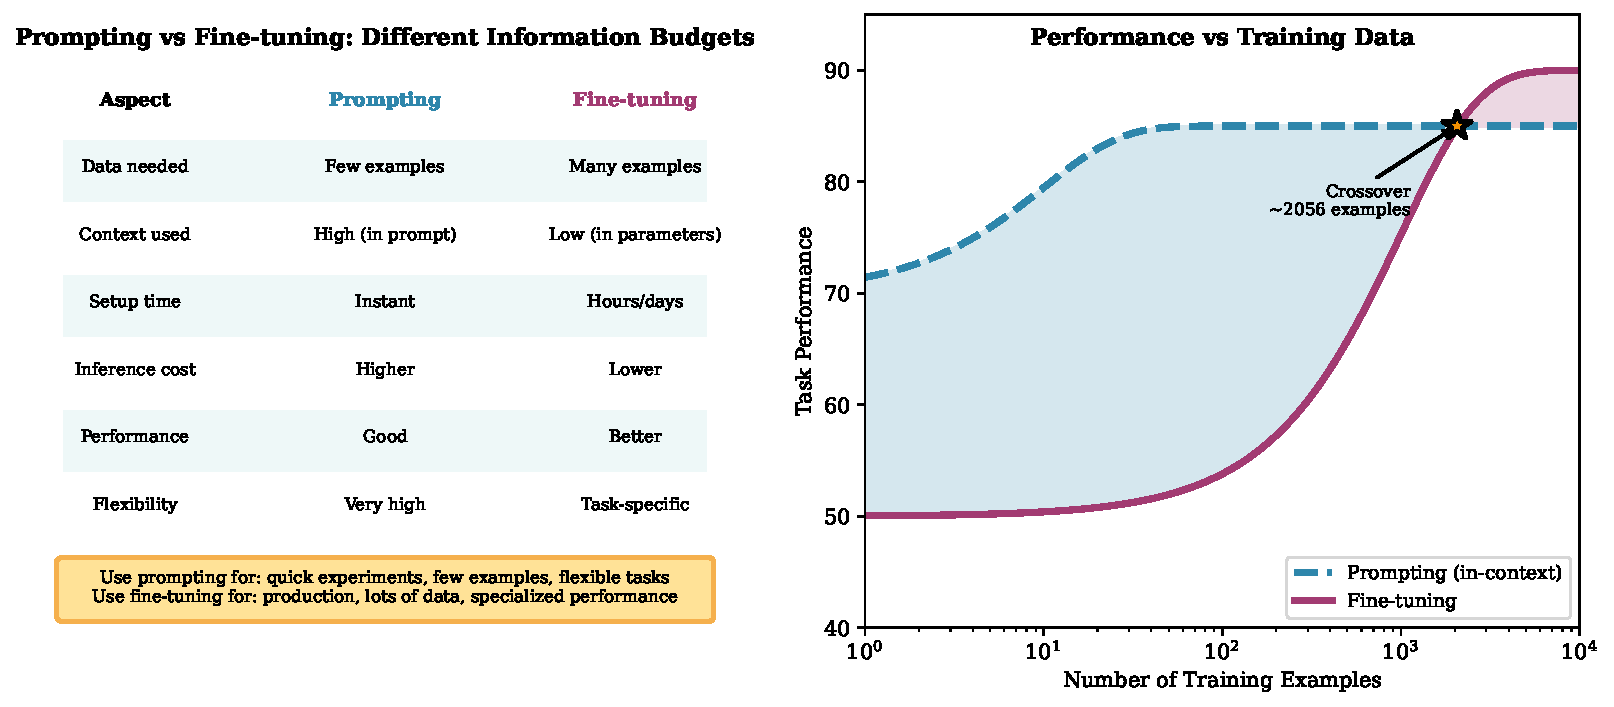
\includegraphics[width=\linewidth]{code/figures/ch06_representation_learning/fig_6_11_prompting_vs_finetuning.pdf}
\caption{Prompting provides task information in-context at inference time; fine-tuning encodes task information in parameters ahead of time.}
\label{fig:prompting_vs_finetuning}
\end{figure}

\vspace{1.5em}


\vspace{1.5em}

\subsection{Monitoring Representations During Training}

Understanding representations also helps with monitoring training. Instead of only watching loss curves, we can track how representations evolve.

Early in training, representations are noisy and high-entropy. Features are not yet separated, and the model has not discovered structure. As training progresses, representations sharpen: features become more distinct, attention patterns become more structured, and entropy decreases.

Here ``entropy'' can be measured directly from attention weights: compute the Shannon entropy of each head's attention distribution and average over tokens. And ``sharpening'' can be operationalized by simple, testable proxies: probe accuracy improves, attention becomes more focused in specialist heads, and representations stabilize over checkpoints (e.g., the same token's hidden state changes less over time on a fixed evaluation set).

We can measure this by tracking probe accuracy over training. If syntactic probes improve while semantic probes lag, the model is learning syntax before semantics. If attention entropy decreases in certain heads, those heads are specializing. These signals complement loss curves and help diagnose training issues.

\vspace{1em}

For example, if loss decreases but representations remain unstructured (high probe error, high entropy), the model might be memorizing rather than learning generalizable features. This suggests overfitting or insufficient regularization. Conversely, if representations sharpen but loss plateaus, the model might need more capacity or a better optimization strategy.

\vspace{1.5em}

\begin{figure}[t]
\centering
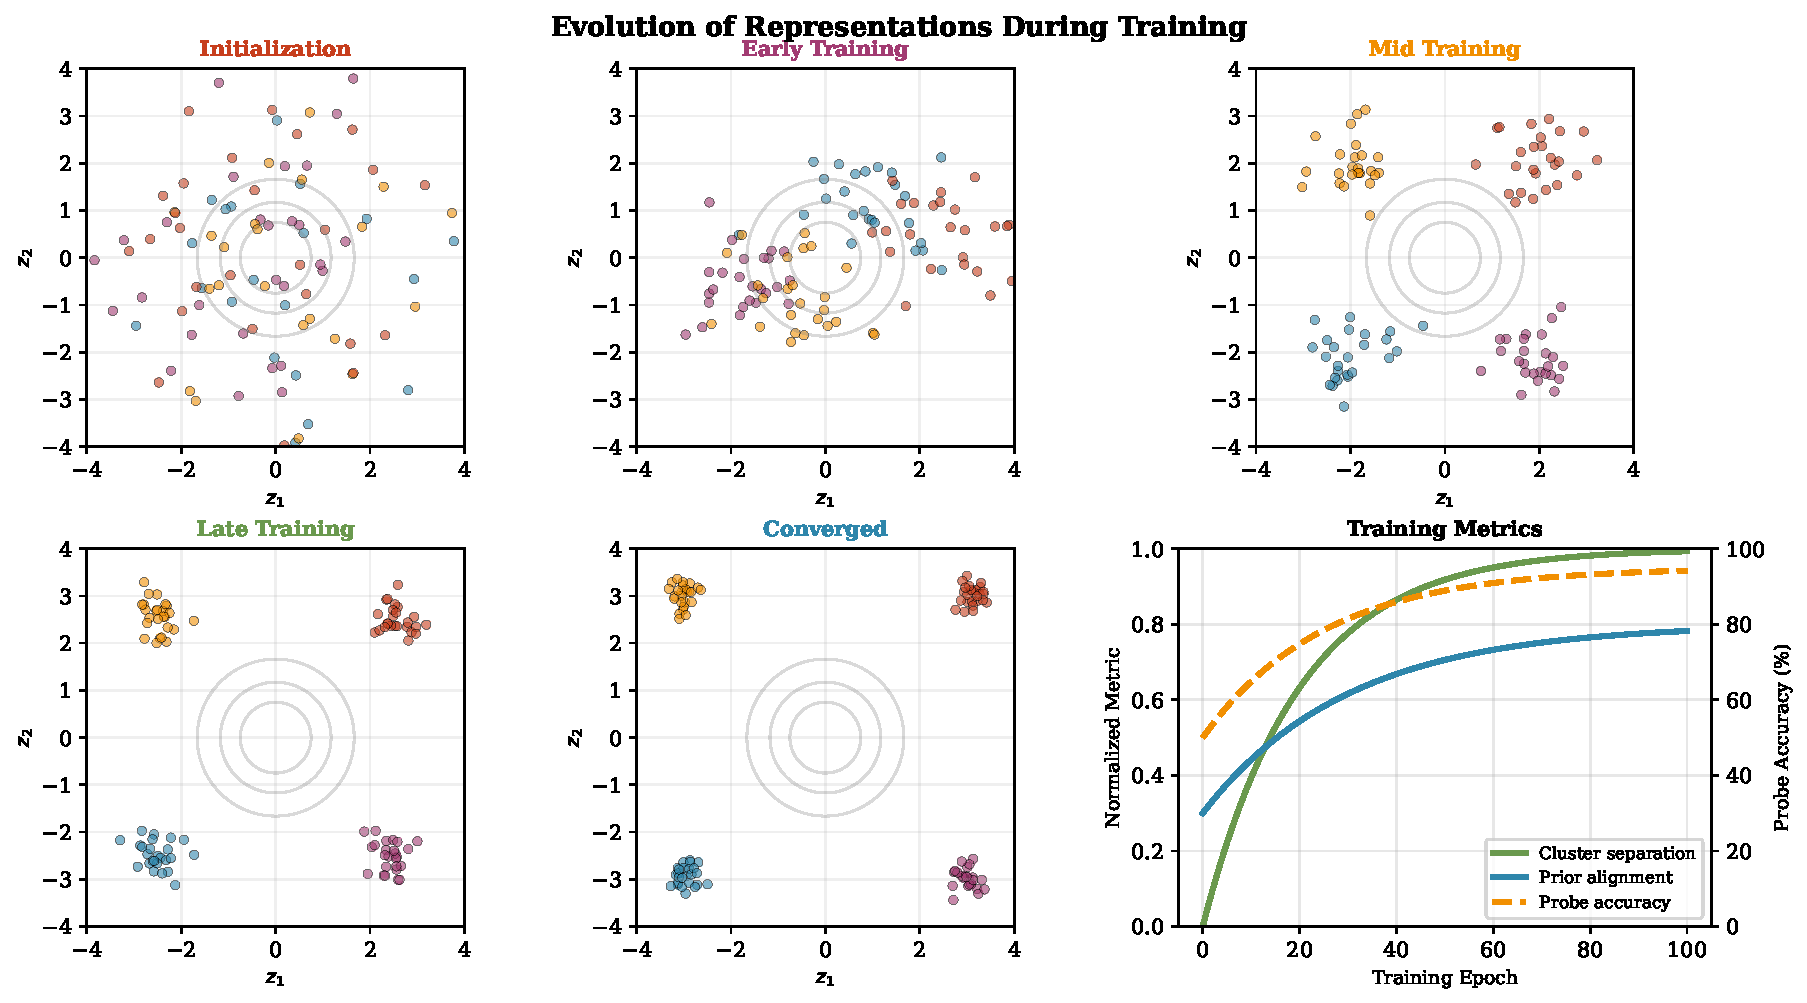
\includegraphics[width=\linewidth]{code/figures/ch06_representation_learning/fig_6_12_training_dynamics.pdf}
\caption{Training dynamics: cluster separation improves, prior alignment stabilizes, and probe accuracy rises over training. Monitoring these alongside loss curves helps diagnose training health.}
\label{fig:training_dynamics}
\end{figure}

\vspace{1.5em}


\vspace{2em}

Pause and reflect. We have seen how understanding representations guides practical decisions: where to fine-tune, how to transfer learning, when to use prompting versus fine-tuning, and how to monitor training. These are not just theoretical curiosities; they are actionable insights that follow directly from the information-theoretic perspective on representation learning.

\vspace{2em}

%==========================
\section{Notes and Caveats}
\label{sec:representation_notes}
%==========================

\subsection{Superposition, Sparsity, and Packing: A Precise View}

The informal claim that ``in high dimensions we can pack thousands of nearly orthogonal features'' deserves a careful accounting. Two regimes matter in practice: fixed-angle packings on the sphere, and small-coherence (small dot product) dictionaries.

\textbf{Fixed-angle spherical packings.}
Let $\theta \in (0,\tfrac{\pi}{2})$ and consider the largest number $N(d,\theta)$ of unit vectors in $\mathbb{R}^d$ with pairwise angles at least $\theta$ (equivalently, pairwise inner products $\le \cos\theta$).
Even coarse volume (sphere-cap) arguments show that for any fixed $\theta$, $N(d,\theta)$ grows exponentially with $d$: $N(d,\theta)=\exp(\Theta(d))$. Sharper upper bounds and constructive lower bounds are studied in spherical coding \citep{kabatiansky1978,delsarte1977}; the key message for our purposes is simply that \emph{fixed} angular margins permit exponentially many directions. This is the regime implicitly invoked when we say ``you can pack thousands of nearly-orthogonal vectors'' in $d\approx 1000$.

\textbf{Small-coherence dictionaries.}
When we demand very small absolute inner products $\mu \stackrel{\mathrm{def}}{=} \max_{i\neq j} |u_i^\top u_j|$, the \emph{Welch bound}~\citep{welch1974} shows that
\[
  \mu^2 \;\ge\; \frac{M-d}{d(M-1)} \qquad \text{for $M$ unit vectors in $\mathbb{R}^d$.}
\]
In particular, once $M$ is appreciably larger than $d$, the right-hand side is $\approx 1/d$, so $\mu$ cannot be much smaller than $1/\sqrt{d}$ no matter how cleverly you choose the vectors. Highly structured constructions (e.g., equiangular tight frames, when they exist) can meet the Welch bound; in real spaces their size is at most on the order of $d^2$. The takeaway is that claims of extremely large catalogs with \emph{vanishing} coherence require care. In practice, modern networks often operate in a regime closer to fixed-angle overlap than to near-zero dot products, and rely on sparsity for reliable readout.
\textbf{Why sparsity saves us.}
Superposition is tractable in deployment because \emph{most features are inactive most of the time}. If only $k$ features are simultaneously active, a $d$-dimensional code with a sufficiently \emph{incoherent} dictionary can still support a huge catalog: under standard Restricted Isometry (RIP)/compressed-sensing conditions \citep{candes2006,donoho2006,baraniuk2007}, a random $d\times n$ dictionary preserves all $k$-sparse signals provided
\[
  d \;\gtrsim\; C\, k \log\!\frac{n}{k}
\]
for a modest constant $C$. Equivalently, with $d=1024$ and $k=16$, this scaling suggests room for $n$ in the tens of millions under idealized assumptions. These results justify the intuition in Section~6.4: superposition can work because \emph{few} features co-activate per input, not because all pairwise dot products are tiny.
\textbf{A toy becomes honest.}
The three-features-in-two-dimensions picture is a didactic metaphor. Real models face far harsher capacity trade-offs: thousands of potential features, modest angles between directions, and varying sparsity across inputs. The right conclusion is not that geometry ``magically'' eliminates interference, but that (i) separation at a fixed angle scales well with dimension, and (ii) sparsity and incoherence allow accurate readout despite superposition.
\begin{examplebox}
\textbf{Back-of-the-envelope.} Suppose a layer activates about $k\!=\!8$ semantic features per token on average, uses $d\!=\!768$ dimensions, and we model its feature directions as roughly random. The $d \gtrsim C k \log(n/k)$ heuristic yields $\log(n/k) \lesssim d/(Ck)\approx 96/C$. Even for $C\!\approx\!5$, this allows $n$ in the millions. The precise constants depend on readout noise, training data, and how ``random'' the dictionary actually is, but the scaling explains why superposition can be practical.
\end{examplebox}
\textbf{What we are (and are not) claiming.}
We are \emph{not} claiming that networks realize optimal spherical codes or satisfy RIP deterministically. We are claiming that the combination of (a) high dimension with \emph{fixed} angular margins, and (b) sparse co-activation, explains why interference can be small enough for linear probes/heads to work.
\textbf{Pointers for the curious.}
Sphere packings and spherical codes \citep{kabatiansky1978,delsarte1977}. Random projections and distance preservation \citep{johnson1984}. Welch bounds \citep{welch1974}. Compressed sensing \citep{candes2006,donoho2006,baraniuk2007}. Sparse coding \citep{olshausen1996}. Mechanistic interpretability work on induction-like circuits and superposition provides empirical context \citep{elhage2021circuits,olsson2022icl}.
\textbf{Caveat (evidence and uncertainty).}
Much of the above is \emph{theoretical scaffolding} for observed behavior in large models. Empirical robustness varies by architecture and scale. Where this chapter speaks causally (``representations emerge from compression''), read it as \emph{pressure and incentive}, not a uniqueness theorem; alternative minima and architectural biases can lead to different representational choices.

\vspace{1em}
\subsection{Empirical Evidence, Probing Debates, and Causal Caveats}

This chapter adopts an information-theoretic lens. Where we use causal shorthand (``representations emerge from compression''), read it as \emph{incentive and pressure}, not uniqueness. Alternative minima and architectural biases can produce different representational choices. We summarize empirical evidence, active debates, and where the theory is still under construction.
\textbf{Empirical anchors (selected).}
A non-exhaustive guide to findings that ground common claims about layerwise structure:
\begin{itemize}
\item \emph{Surface $\rightarrow$ syntax $\rightarrow$ semantics pipeline.} Analyses of BERT-like encoders report that early layers emphasize lexical/surface cues, mid-layers track syntax, and later layers support semantics and task heads \citep{tenney2019pipeline,jawahar2019structure,rogers2020bertology}.
\item \emph{Syntactic geometry.} Structural probes show that distances in representation space can encode parse-tree structure \citep{hewitt2019structural}, though what the model \emph{uses} remains debated (see probing discussion below).
\item \emph{Attention circuits and induction heads.} Mechanistic work isolates ``induction heads'', which are attention patterns that copy and extend token sequences, as one route to in-context learning in decoder-only transformers \citep{elhage2021circuits,olsson2022icl}. Scope across scales/architectures is an active topic.
\item \emph{FFNs as memory/feature stores.} Feed-forward blocks often act like key--value memories that store features retrieved by attention \citep{geva2021kv}, consistent with the superposition picture in Section~6.4.
\item \emph{Scaling, phase changes, and grokking.}\newline Sudden sharpening and late generalization (``grokking'') have been linked to compression dynamics \citep{power2022grokking}; precise triggers vary with data and regularization.
\end{itemize}
\textbf{Probing: what are we really measuring?}
Probing a frozen model with a supervised decoder can reveal \emph{linearly readable} structure, but at least three issues complicate interpretation:
\begin{enumerate}
\item \emph{Amnesic/causal probing.} Probes may learn to reconstruct labels even if the representation does not \emph{causally} contain the feature \citep{ravichander2020probes}. Intervention-based probes and causal ablations help, but are imperfect.
\item \emph{Coordinate dependence.} Linear separability is basis-dependent: a feature can be ``secretly linear'' after a rotation. Control tasks and invariance checks are standard defenses against false positives \citep{belinkov2019survey}.
\item \emph{Use vs.\ presence.} A model might contain information that is not \emph{used} at inference time. Correlating probe-readability with targeted ablations/rule-outs is stronger evidence of use.
\end{enumerate}
\noindent Bottom line: probe scores are informative about \emph{readability}, not definitive about \emph{mechanism}. Good practice layers control tasks, interventions, and task-side ablations.
\textbf{Information bottleneck, honestly.}
The IB Lagrangian, $\min_{p(z|x)} I(X;Z) - \beta I(Z;Y)$, is a useful conceptual scaffold for compression under predictive constraints. The precise connection between IB optimality and gradient-based pretraining of large transformers, however, is unsettled. Competing empirical reports exist on whether mutual information estimates follow canonical IB ``phases''; estimation itself is delicate in high dimensions. Practical stand-ins (rate--distortion views, ELBOs, and signal-to-noise analyses) often provide more stable diagnostics. For deeper treatments see classic IB work \citep{tishby1999ib}, variational IB \citep{alemi2016vib}, and critiques/replications \citep{saxe2019ib}.
\textbf{Further reading (starting points).}
\citep{tenney2019pipeline,jawahar2019structure,rogers2020bertology,hewitt2019structural,elhage2021circuits,olsson2022icl,geva2021kv,ravichander2020probes,belinkov2019survey,tishby1999ib,alemi2016vib,saxe2019ib}.




\section{Looking Forward}
\label{sec:looking_forward}
%==========================

\vspace{1em}

This chapter explored what transformers learn when trained to compress sequences. We saw that representations are not incidental byproducts: when prediction is hard and capacity is limited, training pressure strongly encourages internal structure. Models benefit from discovering patterns that reduce uncertainty, and those patterns can manifest as interpretable regularities in hidden states.

We traced information flow through layers, seeing how depth can create a hierarchy of abstraction from surface statistics to semantic meaning. We examined how attention heads can specialize into functional modules, including induction-like heads for pattern copying, syntactic heads for structure tracking, and semantic heads for conceptual bridging. We explored superposition, a mechanism by which models can pack more potential features than dimensions by tolerating controlled interference in high-dimensional space.

We discussed how to measure representations through probes, interventions, and information-theoretic tools, acknowledging that access matters as much as content. Finally, we connected these insights to practice: understanding representations guides transfer learning, fine-tuning strategies, and training monitoring.

\vspace{1em}

The through-line is that information theory (and, when useful, an information-geometry view of predictive distributions) provides a coherent way to think about representation learning. Many qualitative regularities, such as layerwise hierarchies, specialization, and superposition, can be understood as efficient responses to predictive objectives under constraints, even though the details are not unique and vary across architectures and scales.

In Chapter 7, we will shift from discrete autoregressive models to continuous diffusion models. The questions change, including how you compress images rather than text and how you generate by denoising rather than by sequential prediction, but the information-theoretic principles remain the same. Compression, structure discovery, and rate-distortion tradeoffs continue to guide us as we explore different modeling paradigms.

\vspace{1em}

\begin{pausebox}
\textbf{Chapter Summary.} Representations are shaped by compression pressure. Training transformers to predict text encourages them to capture statistical structure such as syntax, semantics, and composition, and encode it efficiently in fixed-width vectors. This can produce a hierarchy of abstraction across layers, functional specialization within attention heads, and superposition under capacity constraints. Understanding these representations through an information-theoretic lens helps guide practical decisions about transfer learning, fine-tuning, and model usage.
\end{pausebox}

\vspace{2em}
